\chapter{Implementierung der Webanwendung}

Die AnwenderInnen sollen zu Beginn Datensätze anlegen können. Im Prototypen wurde das Datenmodell von Personen mit Benutzername, E-Mail und Passwort herangezogen.
Nachdem die AnwenderInnen das Formular für eine Person ausgefüllt haben, kann dieser Datensatz angelegt werden. Nach elementaren Validierungen werden die Daten an den Server übermittelt. Dieser speichert diese wiederum in der Datenbank ab. 
In der Listenansicht sehen die AnwenderInnen alle bereits angelegten Personen in einer Tabelle und per Klick auf den Namen wird zur Detailansicht weitergeleitet. Hier wird ein Formular mit den Nutzerdaten ausgefüllt, welche verändert und aktualisiert werden können.   
Auf der Detailseite findet sich ebenso ein Lösch-Knopf, um eine bestehende Person zu entfernen. Dadurch sind alle CRUD-Operation abgedeckt.
\section{Voraussetzungen für die Webanwendung}
Um die Nutzung von Webkomponenten am Server zu ermöglichen, werden zwei konkrete Technologien benötigt, da Webkomponenten grundsätzlich nur im Browser funktionieren.
\subsection{Electron}
Electron ist ein Framework, um native Cross-Plattform-Applikationen mit Web-Technologien wie Javascript, HTML und CSS zu erstellen. Es basiert auf dem Chromium\footnote{https://www.chromium.org/} Webbrowser und Node.js.
\subsection{Scram-Engine}
\label{cha:scram-engine}
Das Scram-Engine-Projekt, erarbeitet von Jordan Last, ermöglicht es, eine HTML-Datei einem vorkonfigurierten Electronstartscript mit minimalem Aufwand zur Verfügung zu stellen. Es wird lediglich Electron von der Kommandozeile aufgerufen und eine Startdatei mitgegeben. Die Vorkonfiguration vereinfacht das Arbeiten mit Electron durch beispielsweise das Anbieten von Kommandozeilenargumenten, um das Electronfenster zu verstecken, und somit das bequeme Starten von serverseitigen Anwendungen aus der Kommandozeile heraus.
Electron ist notwendig, da es Chromium mit Node.js kombiniert. Die Scram-Engine nutzt Chromiums Fähigkeit, Webkomponenten in einen interaktiven DOM zu parsen, welcher manipuliert werden kann. Diese Webkomponenten können dadurch jeglichen Node.js Code nutzen und haben die Möglichkeit mit dem Betriebssystem zu interagieren, Datenbankaufrufe zu tätigen, prinzipiell alles, was Node.js möglich ist.
Ein reiner Node.js Server würde nicht ausreichen, da dieser HTML, Custom-Elemente oder Webkomponenten generell nicht parsen kann.
Durch die Kombination der beiden Technologien können Webkomponenten weitaus mehr leisten, als in einem Webbrowser.

Da universelle Webkomponenten auf Electron als deren Plattform angewiesen sind, muss das System, welches diese betreibt, relativ leistungsstark sein. Jordan Last arbeitet an einer Lösung, um die Electron-Abhängigkeit -- und dadurch die Chromium-Abhängigkeit -- loszuwerden\footnote{https://github.com/lastmjs}.

\section{Implementierung der Komponenten}
Der für diese Arbeit entwickelte Prototyp kann in die Hauptteile Frontend und Backend eingeteilt werden. Wobei das Backend nochmals in Server und Datenbank unterteilt wird. 

\subsection{Frontend}
Im Frontend wurde hauptsächlich auf bereits vorhandenen Webkomponenten aufgebaut. Es wurden Standard HTML-Elemente durch paper-input Elemente\footnote{https://www.webcomponents.org/collection/PolymerElements/paper-input-elements} ersetzt, um ein abgestimmtes Gesamtbild zu erzeugen, ohne sich auf das Design konzentrieren zu müssen. So wurde bei dem Anlegen einer neuen Person, wie in Abb. \ref{fig:user_create} ersichtlich, auf <paper-input> Elemente mit einem <iron-icon> Element gesetzt. Das Aktualisieren eines Nutzers ist das selbe Formular, lediglich mit anderen <paper-button> Komponenten. Die Auflistung aller bereits erstellten Personen wurde durch ein <paper-datatable-api> Element erstellt. Jegliche Kommunikation zwischen Frontend und Backend wurde über eine REST-API gehandhabt. Die Anfragen wurden durch <iron-ajax> Komponenten vollzogen, welche eine Webkomponente für einfache ajax-Anfragen ist.
\begin{figure}
	\centering
	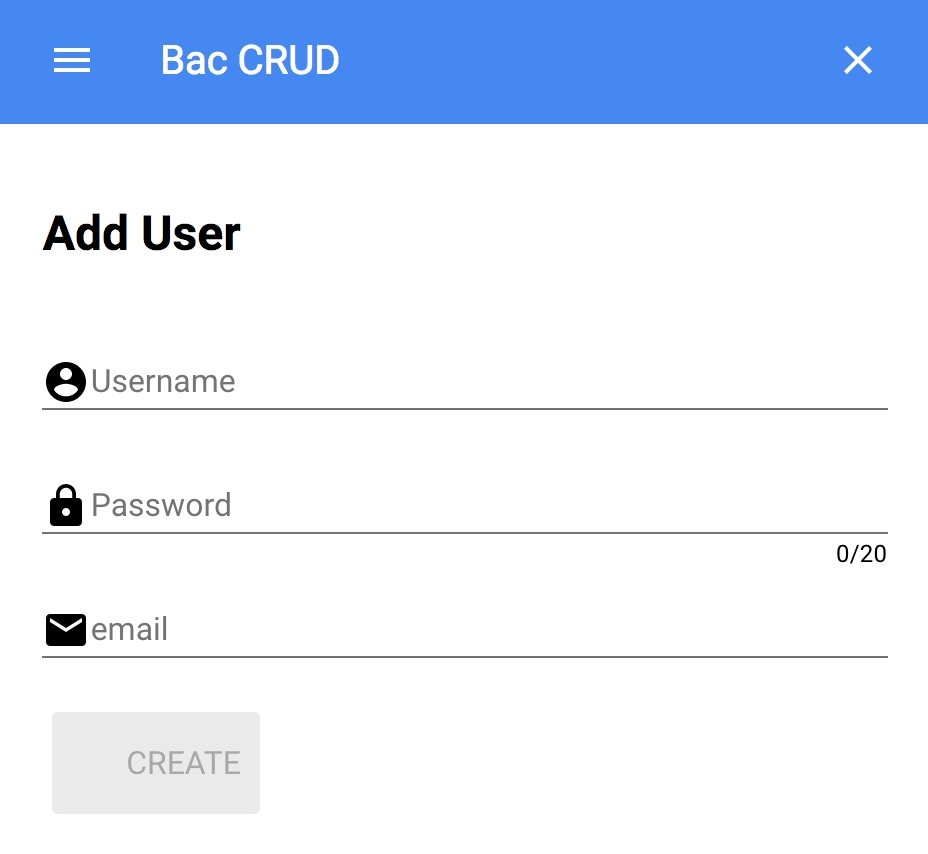
\includegraphics[width=0.5\linewidth]{images/user_create.jpeg}
	\caption{User erstellen}
	\label{fig:user_create}
\end{figure}

\begin{figure}
	\centering
	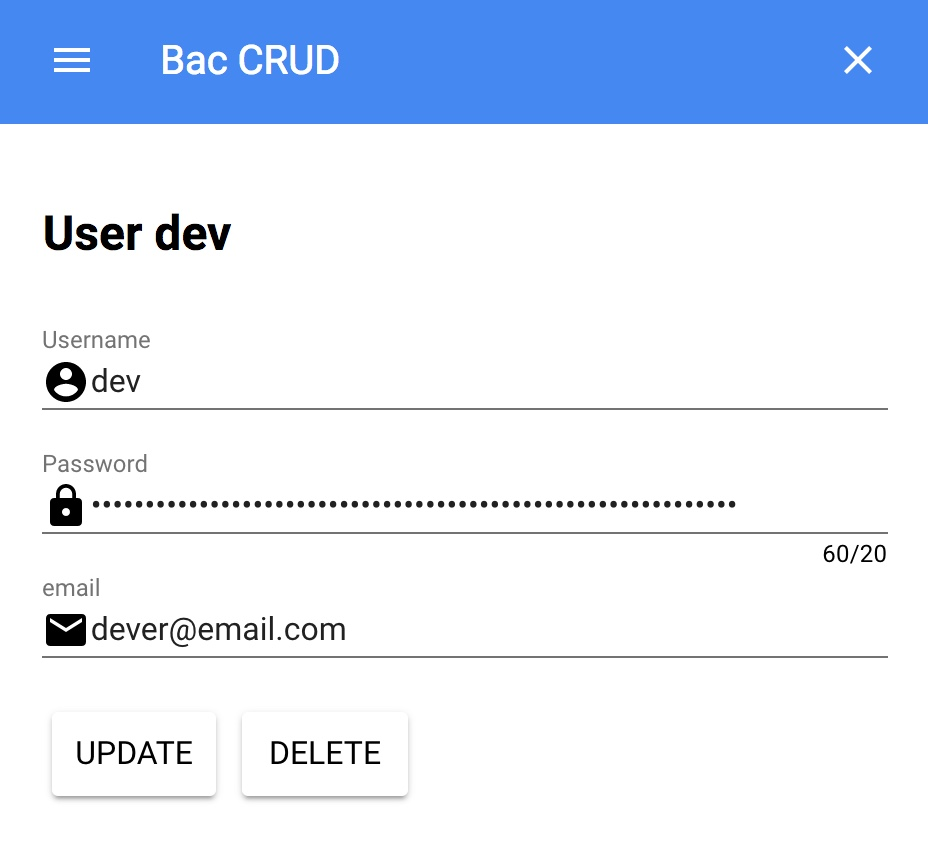
\includegraphics[width=0.5\linewidth]{images/user_update.jpeg}
	\caption{User bearbeiten}
	\label{fig:user_update}
\end{figure}

\begin{figure}
	\centering
	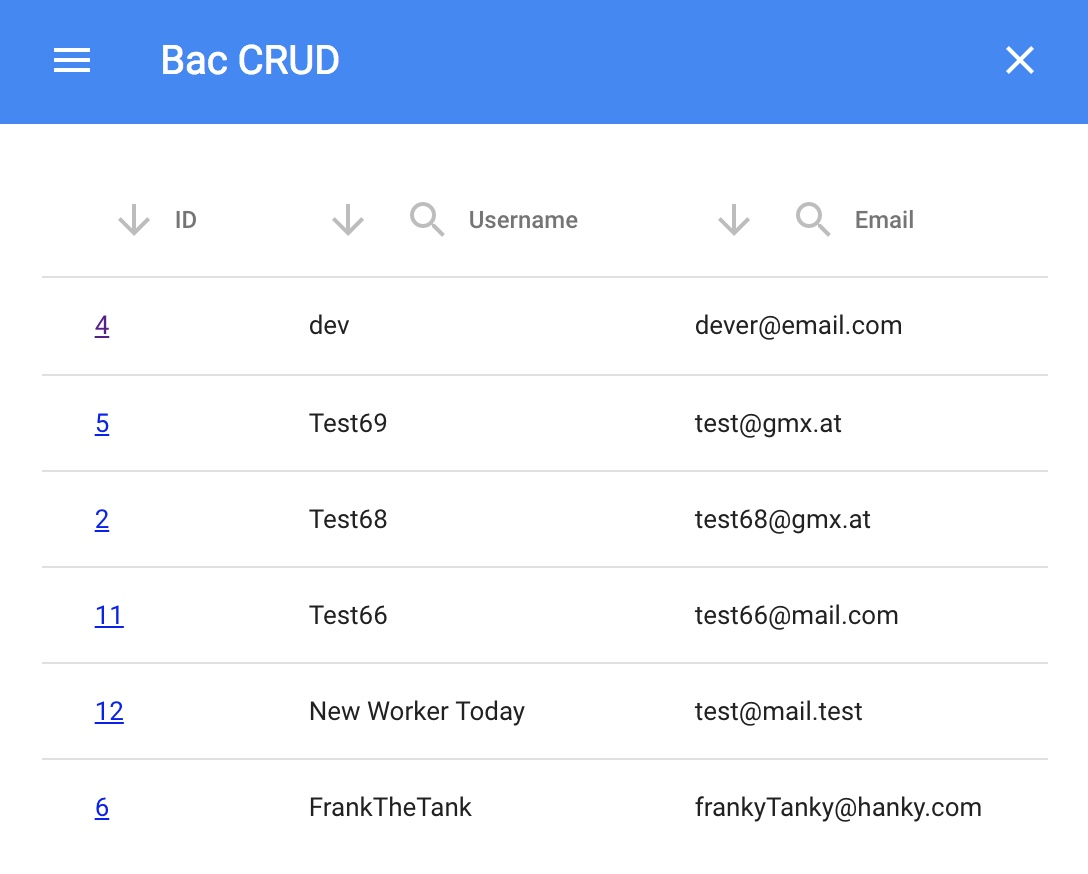
\includegraphics[width=0.5\linewidth]{images/user_list.jpeg}
	\caption{User Liste}
	\label{fig:user_list}
\end{figure}

\subsection{Server}
Ein Node.js Server kann mit Webkomponenten, wie im Programm \ref{prog:server-config} abgekürzt ersichtlich, konfiguriert und funktionstüchtig eingesetzt werden. Durch <express-app>, <express-config>, <express-middlesware> und <express-router> mit <express-route> Komponenten\footnote{https://github.com/scramjs/express-web-components} kann die komplette Serverumgebung aufgesetzt werden.

In dieser Serveranwendung sind alle Endpunkte und Middlewares, welche die Express-Anwendung manipulieren, unter einer <express-app> Webkomponente  verschachtelt. In der Reihenfolge, wie die Middlewares definiert werden, werden diese auch in die Anwendung eingepflegt. In einem <express-router> Element können ebenfalls <express-route> Elemente und Middlewares verschachtelt, und so komplexe Routen-System erstellt werden.

Anstatt REST-Routen in Javascript imperativ zu definieren, können diese deklarativ in HTML zusammengesetzt werden. Es wird so eine visuelle Hierarchie der vorhanden Routen erstellt. Durch die Visualisierung mit HTML behält man nicht nur den Überblick, es ist auch einfacher zu verstehen als das Äquivalent in Javascript. Hier wird beispielsweise im Programm \ref{prog:route-config} der \textit{indexHandler}(siehe Programm \ref{prog:indexHandler}) als \textit{Callback} an ein <express-middleware> Element übergeben, welches eine Methode(\textit{get}) und einen Pfad(\textit{/})  besitzt. Diese Middleware befindet sich unter dem <express-router> mit der Basisroute als Pfad. Das bedeutet, dass dieser Router für seinen Pfad unter sich Routen haben kann, die ebenso einen Pfad besitzen. Da der \textit{indexHandler} auf die Basisroute angewendet werden soll, wird dieser Middleware ebenfalls die Basisroute als Pfad mitgegeben. Nach diesem Prinzip können jegliche verschachtelte Routen erstellt werden. Wobei Subrouten immer unter der übergeordneten Route verschachtelt werden sollen. So soll die Route \textit{/index/list} unter dem Router für die Route \textit{/index} als Route \textit{/list} geschachtelt werden.

Die gezeigte Route im Code  \ref{prog:route-config} ist rein zur Definition, welche URL welche Seite rendern soll. Für REST-Anfragen, die Daten aus der Datenbank manipulieren, wurde eine eigene Komponente <db-router> erstellt, welche alle relevanten Datenbankanfragen über zuvor definierte Routen verarbeitet. Diese Komponente, welche selbst <express-router> Elemente implementiert, kapselt so datenbank-spezifische Endpunkte von der Serverkonfiguration ab. Dieser <db-router> ist, ebenso wie ein <express-router> Element, ein Kind der <express-app> Komponente. Ersichtlich im Programm \ref{prog:server-config}.

\begin{program}
\caption{Exemplarische Express-App mit Webkomponenten}
\label{prog:server-config}
\begin{HtmlCode}
<express-app port="3000">
	<express-config callback="[[staticMW]]"></express-config>
	<express-middleware callback="[[bodyParserMW]]"></express-middleware>
	<express-router path="/">
	<express-middleware method="get" path="/" callback="[[indexHandler]]"></express-middleware>
	</express-router>
	<db-router></db-router>
</express-app>
\end{HtmlCode}
\end{program}

\begin{program}
\caption{Indexroute-Konfiguration mit Webkomponenten}
\label{prog:route-config}
\begin{HtmlCode}
<express-router path="/">
	<express-middleware method="get" path="/" callback="[[indexHandler]]"></express-middleware>
</express-router>
\end{HtmlCode}
\end{program}

\begin{program}
\caption{indexHandler Funktion}
\label{prog:indexHandler}
\begin{HtmlCode}
indexHandler(req, res) {
	res.sendFile(path.resolve('./client/index.html'));
}
\end{HtmlCode}
\end{program}

\subsection{Datenverwaltung}
Der im Programm \ref{prog:server-config} ersichtliche <db-router> verarbeitet jegliche datenbank-spezifischen Anfragen und triggert <db-query> Komponenten, um Daten der Datenbank zu manipulieren. Siehe Programm \ref{prog:db-query}. Diesem <db-query> Element wird durch Kindelemente mitgeteilt, welche Abfragen es tätigen soll. Besitzt das <db-query> Element beispielsweise lediglich ein <db-find> Element, wird davon ausgegangen, dass ein Datensatz von der Datenbank gesucht und zurückgegeben werden soll. Besitzt es aber zusätzlich zu dem <db-find>, ein <db-delete>, so wird das <db-query> Element nicht den gefunden Datensatz zurückgeben, sondern löschen. 
 
\begin{program}
\caption{Datenverwaltung mit Komponenten}
\label{prog:db-query}
\begin{HtmlCode}
<db-query id="queryListUsers" db-model="[[userModel]]">
	<db-find></db-find>
	<db-sort sort2-query="{{_sort}}" sort-query="[[_sort]]" sort-property="username"
		sort-direction="asc"></db-sort>
</db-query>
	
<db-query id="queryUserDetails" db-model="[[userModel]]">
	<db-find find-query="[[findUserQuery]]"></db-find>
</db-query>
	
<db-query id="querySaveUser" db-model="[[userModel]]">
	<db-save save="[[newUser]]"></db-save>
</db-query>
	
<db-query id="queryUpdateUser" db-model="[[userModel]]">
	<db-find find-query="[[findUserQuery]]"></db-find>
	<db-save save="[[updateUser]]"></db-save>
</db-query>
	
<db-query id="queryDeleteUser" db-model="[[userModel]]">
	<db-find find-query="[[findUserQuery]]"></db-find>
	<db-delete></db-delete>
</db-query>
\end{HtmlCode}
\end{program}

\subsubsection{DB Query Komponente}
Um die interne Arbeitsweise zu verdeutlichen, wird die im Zuge dieser Arbeit entwickelte Webkomponente erläutert. Der exakte Programmcode kann auf GitHub nachgelesen werden\footnote{https://github.com/drdreo/webcomponent-cms/blob/master/server/components/db-query.html}.
Als Parameter benötigt das <db-query> Element eine eindeutige ID, welche zum Auslösen der Abfrage verwendet wird, und das zugehörige  Datenbankmodell -- da dieses Element für mongoDB mit mongoose entworfen wurde.

Im Programm~\ref{prog:db-query-implementation} wird die gekürzte Version der Implementierung gezeigt. Es wurden einige Programmteile herausgenommen, da diese nicht wesentlich zum Verständnis beitragen würden, und lediglich den Code verlängern.

Die Komponente ist so konzipiert, dass diese zu Beginn durch alle Kindelemente traversiert, die unterschiedlichen Typen überprüft und abhängig von den vorhanden DB-Element-Typen\footnote{DB wurde als Präfix für die Datenbank Webkomponenten gewählt} die Element-Parameter zur eigentlichen \textit{Query} zusammenfügt. Mit einer Funktion(\textit{execute}), siehe Programm~\ref{prog:db-query-execute}, welche als Parameter eine Callback-Funktion mitbekommt, kann die  \textit{Query} ausgelöst und auf das Resultat reagiert werden.

Im Programm~\ref{prog:db-query} ist beispielsweise ersichtlich, dass bei einer \textit{delete-Query} (\textit{id = queryDeleteUser}) ein \textit{find-Element} vorhanden sein muss, und ein leeres \textit{delete-Element}. Dadurch wird dieser \textit{DB-Query-Komponente} mitgeteilt, das sie diese \textit{find-Query} ausführen, und den gefundenen Datensatz entfernen soll.
\begin{program}
	\caption{DB-Query Implementierung}
	\label{prog:db-query-implementation}
	\begin{HtmlCode}
 class DbQuery extends HTMLElement {
	 	
	 	{...}
	 	
	 	initChildren(){
	 		// iterate through db children and set query parameters
	 		this._children.forEach((child) => {
	 			// db-find element, get query attribute, check if the attribute has value
	 			if (child.nodeName === "DB-FIND") {
	 				if (child.findQuery) // JSON object query
	 				{
	 					this.findQuery = child.findQuery;
	 				}
	 				this.queryType = "find";
	 			}
	 			// db-delete element
	 			if (child.nodeName === "DB-DELETE") {
	 				this._delete = true;
	 				this.queryType = "delete";
	 			}
	 		});
	 	}
	 	
	 	execute(callback){
	 		this.initChildren();
	 		const find = this.findQuery;
	 		switch (this.queryType) {
	 			case "find":
		 			this.dbModel.find(find).exec(function (err, results) {
		 				callback(err, results);
		 			});
	 			break;
	 			case "delete":
		 			this.dbModel.remove(find).exec(function (err, doc) {
		 				callback(err, doc);
		 			});
	 			break;
	 		}
	 	}
 }
\end{HtmlCode}
\end{program}

\begin{program}
\caption{Auslösen einer DB-Query-Komponente}
\label{prog:db-query-execute}
\begin{HtmlCode}
this.shadowRoot.getElementById("queryDeleteUser").execute(function (err, user) {
	res.json("User deleted successfully.");
});
\end{HtmlCode}
\end{program}
